\SourceLeaf{301}ten kleinen Kreise unabhängig; also der Inhalt von $ABC$ für jede Lage von $C$ in diesem kleinen Kreise immer derselbe. Für den Fall, wo $\gamma$ nicht innerhalb des Dreiecks liegt, muss man (wie das bei synthetischen Beweisen immer nothwendig ist) eine andere Figur zeichnen, welche zeigt, dass sowohl das Dreieck $ABC$, als das Viereck $A\alpha\beta B$ jedes $=1+2+3$ ist.

\begin{center}\resizebox{8.0cm}{!}{%
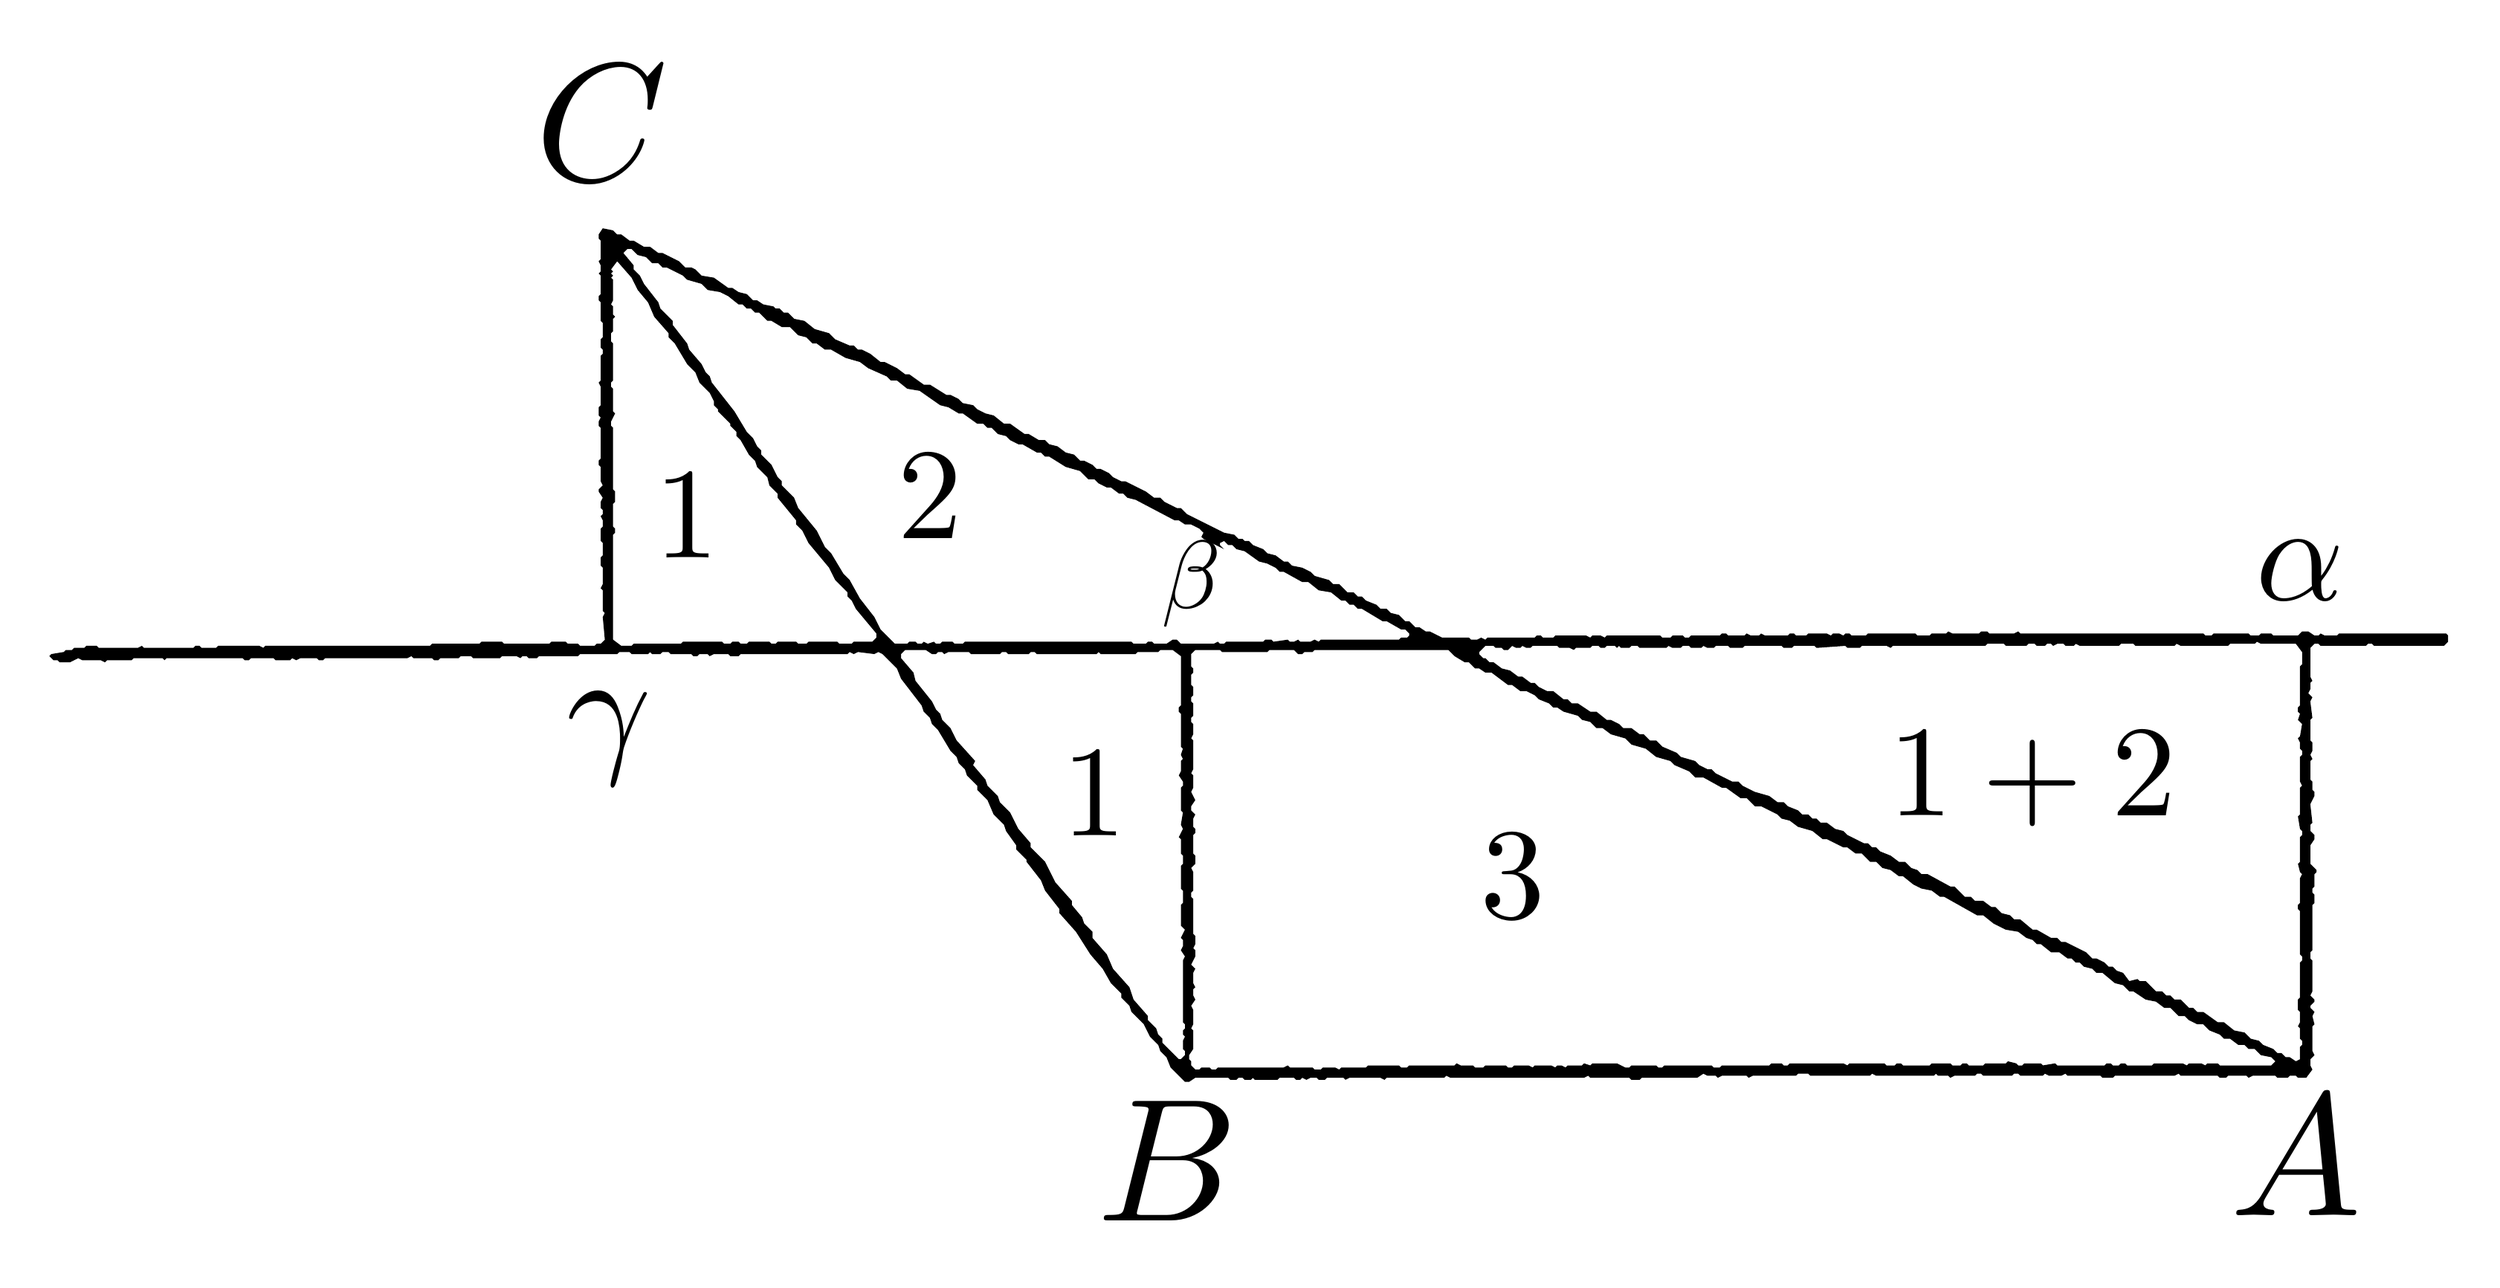
\begin{tikzpicture}[x=1pt,y=-1pt]
\path[use as bounding box] (0,0) rectangle (1195,606);
\path[fill=black,draw=none,even odd rule]
(14,309) -- (16,311) -- (18,311) -- (19,312) -- (24,312) -- (28,310) -- (30,311) -- (39,311) -- (41,312) -- (42,311) -- (54,311) -- (55,310) -- (69,310) -- (70,311) -- (71,310) -- (108,310) -- (109,311) -- (111,311) -- (112,310) -- (123,310) -- (124,311) -- (131,311) -- (132,310) -- (134,311) -- (136,310) -- (144,310) -- (145,311) -- (147,311) -- (148,310) -- (188,310) -- (190,309) -- (191,310) -- (200,310) -- (201,311) -- (203,311) -- (204,310) -- (213,310) -- (214,309) -- (219,309) -- (220,310) -- (233,310) -- (234,309) -- (241,309) -- (243,310) -- (244,309) -- (246,309) -- (247,310) -- (251,310) -- (252,309) -- (271,309) -- (272,308) -- (290,308) -- (291,307) -- (296,307) -- (297,308) -- (305,308) -- (306,307) -- (307,308) -- (311,308) -- (312,307) -- (315,307) -- (316,308) -- (326,308) -- (327,309) -- (329,309) -- (330,308) -- (334,308) -- (335,309) -- (337,308) -- (344,308) -- (345,309) -- (349,309) -- (350,308) -- (402,308) -- (403,307) -- (405,308) -- (407,307) -- (415,308) -- (417,307) -- (419,308) -- (426,315) -- (428,320) -- (438,333) -- (439,336) -- (442,339) -- (443,342) -- (446,345) -- (452,355) -- (455,358) -- (456,361) -- (459,364) -- (460,367) -- (465,372) -- (465,374) -- (470,379) -- (473,386) -- (478,391) -- (479,394) -- (484,401) -- (484,403) -- (489,408) -- (489,409) -- (496,418) -- (498,423) -- (505,432) -- (505,434) -- (513,443) -- (520,454) -- (526,461) -- (530,468) -- (535,473) -- (535,475) -- (539,479) -- (540,482) -- (546,488) -- (549,494) -- (553,498) -- (554,501) -- (557,504) -- (559,509) -- (566,516) -- (568,516) -- (571,514) -- (587,514) -- (588,515) -- (591,515) -- (592,514) -- (594,514) -- (595,515) -- (598,515) -- (599,514) -- (600,515) -- (611,515) -- (612,514) -- (619,514) -- (620,515) -- (622,515) -- (623,514) -- (625,515) -- (627,514) -- (630,514) -- (631,515) -- (634,515) -- (635,514) -- (643,514) -- (644,515) -- (646,514) -- (661,514) -- (663,515) -- (664,514) -- (692,514) -- (693,513) -- (695,514) -- (760,514) -- (762,513) -- (763,514) -- (782,514) -- (783,515) -- (787,515) -- (788,514) -- (815,514) -- (818,512) -- (820,513) -- (824,513) -- (825,514) -- (827,513) -- (839,513) -- (840,514) -- (842,513) -- (863,513) -- (864,512) -- (869,512) -- (870,513) -- (899,513) -- (900,512) -- (902,513) -- (930,513) -- (931,512) -- (932,513) -- (937,513) -- (938,514) -- (940,513) -- (950,513) -- (951,512) -- (953,512) -- (954,513) -- (968,513) -- (969,512) -- (971,512) -- (972,513) -- (983,513) -- (984,512) -- (986,513) -- (992,513) -- (994,512) -- (995,513) -- (1011,513) -- (1012,514) -- (1017,514) -- (1018,513) -- (1047,513) -- (1049,512) -- (1050,513) -- (1068,513) -- (1069,514) -- (1072,514) -- (1073,513) -- (1082,513) -- (1083,514) -- (1085,513) -- (1096,513) -- (1097,514) -- (1102,514) -- (1103,513) -- (1106,513) -- (1107,514) -- (1111,514) -- (1114,510) -- (1113,508) -- (1113,505) -- (1115,503) -- (1114,501) -- (1114,489) -- (1115,488) -- (1114,484) -- (1115,482) -- (1113,480) -- (1113,479) -- (1115,477) -- (1115,476) -- (1113,474) -- (1114,472) -- (1114,457) -- (1113,456) -- (1113,453) -- (1114,452) -- (1114,430) -- (1115,429) -- (1115,425) -- (1114,424) -- (1114,422) -- (1115,421) -- (1115,415) -- (1116,414) -- (1116,413) -- (1113,410) -- (1113,401) -- (1115,398) -- (1115,396) -- (1113,394) -- (1113,391) -- (1114,390) -- (1113,381) -- (1115,377) -- (1115,375) -- (1114,374) -- (1114,370) -- (1113,369) -- (1113,360) -- (1114,359) -- (1113,357) -- (1114,355) -- (1114,351) -- (1113,350) -- (1113,340) -- (1114,339) -- (1113,331) -- (1114,329) -- (1112,327) -- (1113,325) -- (1113,322) -- (1114,321) -- (1113,319) -- (1113,305) -- (1115,303) -- (1117,303) -- (1118,304) -- (1140,304) -- (1141,303) -- (1143,303) -- (1144,304) -- (1178,304) -- (1180,302) -- (1180,299) -- (1179,298) -- (1127,298) -- (1126,299) -- (1120,299) -- (1118,298) -- (1117,299) -- (1115,299) -- (1112,297) -- (1109,297) -- (1107,299) -- (1095,299) -- (1094,298) -- (1089,298) -- (1088,299) -- (1084,299) -- (1083,298) -- (1066,298) -- (1065,299) -- (1062,299) -- (1061,298) -- (972,298) -- (971,297) -- (969,298) -- (957,298) -- (956,297) -- (953,297) -- (952,298) -- (939,298) -- (937,297) -- (936,298) -- (929,298) -- (928,299) -- (922,299) -- (921,298) -- (898,298) -- (897,299) -- (890,299) -- (889,298) -- (887,298) -- (886,299) -- (884,298) -- (881,298) -- (880,299) -- (878,298) -- (869,298) -- (868,299) -- (863,299) -- (862,298) -- (860,298) -- (859,299) -- (848,299) -- (846,298) -- (845,299) -- (841,299) -- (839,298) -- (838,299) -- (830,299) -- (829,298) -- (827,298) -- (826,299) -- (812,299) -- (811,300) -- (809,300) -- (808,299) -- (803,299) -- (802,300) -- (798,300) -- (797,299) -- (771,299) -- (770,300) -- (768,299) -- (764,299) -- (763,300) -- (761,299) -- (746,299) -- (745,300) -- (740,300) -- (739,299) -- (737,299) -- (736,300) -- (713,300) -- (712,301) -- (710,300) -- (708,301) -- (705,301) -- (704,300) -- (691,300) -- (685,297) -- (683,297) -- (680,295) -- (678,295) -- (675,292) -- (673,292) -- (670,289) -- (666,288) -- (664,286) -- (661,286) -- (659,284) -- (654,282) -- (652,280) -- (650,280) -- (648,278) -- (645,278) -- (641,274) -- (638,274) -- (636,272) -- (629,270) -- (627,268) -- (623,266) -- (618,265) -- (616,263) -- (614,263) -- (610,260) -- (606,259) -- (604,257) -- (599,255) -- (597,253) -- (595,253) -- (594,252) -- (592,252) -- (590,250) -- (585,249) -- (567,240) -- (564,237) -- (562,237) -- (556,234) -- (554,232) -- (551,232) -- (547,229) -- (537,224) -- (535,224) -- (531,222) -- (529,220) -- (525,218) -- (523,218) -- (521,216) -- (517,214) -- (515,214) -- (512,211) -- (508,210) -- (504,207) -- (500,206) -- (498,204) -- (495,204) -- (490,201) -- (488,201) -- (481,196) -- (478,196) -- (473,192) -- (469,191) -- (465,189) -- (463,187) -- (458,186) -- (456,184) -- (452,182) -- (450,182) -- (442,177) -- (439,177) -- (432,172) -- (430,172) -- (426,169) -- (420,166) -- (418,166) -- (413,162) -- (409,160) -- (407,160) -- (405,158) -- (403,158) -- (396,155) -- (393,152) -- (386,150) -- (381,146) -- (376,145) -- (373,142) -- (371,142) -- (369,140) -- (367,140) -- (366,139) -- (361,138) -- (358,136) -- (356,136) -- (353,133) -- (349,132) -- (346,130) -- (344,130) -- (337,125) -- (331,124) -- (328,121) -- (326,120) -- (323,120) -- (320,117) -- (312,113) -- (310,113) -- (306,110) -- (303,110) -- (298,107) -- (296,107) -- (292,104) -- (290,104) -- (288,102) -- (283,101) -- (281,104) -- (281,106) -- (282,107) -- (282,116) -- (281,117) -- (282,119) -- (282,122) -- (281,123) -- (282,124) -- (282,133) -- (281,134) -- (281,136) -- (282,137) -- (282,146) -- (283,147) -- (283,154) -- (282,155) -- (282,159) -- (283,160) -- (283,162) -- (282,163) -- (282,175) -- (281,176) -- (282,178) -- (282,187) -- (281,188) -- (281,192) -- (282,193) -- (281,195) -- (281,197) -- (282,198) -- (282,213) -- (281,214) -- (281,216) -- (282,217) -- (282,224) -- (283,226) -- (281,228) -- (281,229) -- (283,232) -- (282,234) -- (282,237) -- (283,238) -- (283,240) -- (282,241) -- (283,243) -- (283,246) -- (282,247) -- (282,253) -- (283,254) -- (283,260) -- (282,261) -- (282,265) -- (283,266) -- (283,274) -- (282,276) -- (283,277) -- (283,287) -- (284,288) -- (283,290) -- (284,301) -- (282,303) -- (280,303) -- (279,304) -- (272,304) -- (271,303) -- (266,303) -- (265,302) -- (258,302) -- (257,303) -- (235,303) -- (234,302) -- (224,302) -- (223,303) -- (200,303) -- (199,304) -- (119,304) -- (118,305) -- (116,304) -- (96,304) -- (95,305) -- (88,305) -- (87,304) -- (85,304) -- (84,305) -- (60,305) -- (59,304) -- (57,305) -- (38,305) -- (37,304) -- (32,304) -- (31,305) -- (26,305) -- (25,306) -- (22,306) -- (21,307) -- (15,308) -- cycle
(569,308) -- (571,306) -- (583,306) -- (584,307) -- (606,307) -- (607,306) -- (619,306) -- (621,308) -- (623,308) -- (624,307) -- (628,307) -- (629,306) -- (694,306) -- (697,309) -- (702,312) -- (704,312) -- (707,315) -- (709,315) -- (712,317) -- (715,317) -- (723,323) -- (725,323) -- (729,326) -- (732,326) -- (736,328) -- (738,330) -- (743,332) -- (745,334) -- (747,334) -- (750,336) -- (757,338) -- (759,340) -- (763,341) -- (766,344) -- (769,344) -- (773,347) -- (780,349) -- (783,352) -- (790,354) -- (795,358) -- (802,360) -- (804,362) -- (811,365) -- (814,368) -- (818,368) -- (827,373) -- (829,373) -- (836,378) -- (839,378) -- (843,382) -- (846,382) -- (854,386) -- (856,388) -- (860,389) -- (864,392) -- (871,394) -- (876,398) -- (878,398) -- (886,402) -- (888,402) -- (892,405) -- (895,405) -- (899,409) -- (902,409) -- (905,412) -- (909,413) -- (913,416) -- (915,416) -- (920,420) -- (924,422) -- (929,423) -- (933,426) -- (935,426) -- (951,435) -- (954,435) -- (959,439) -- (965,442) -- (971,443) -- (975,446) -- (978,447) -- (980,449) -- (982,449) -- (987,453) -- (991,453) -- (995,456) -- (997,456) -- (999,458) -- (1001,458) -- (1003,460) -- (1007,461) -- (1009,463) -- (1012,463) -- (1018,468) -- (1022,469) -- (1025,472) -- (1027,472) -- (1033,476) -- (1038,477) -- (1042,480) -- (1045,480) -- (1049,484) -- (1052,484) -- (1054,486) -- (1058,488) -- (1061,488) -- (1064,491) -- (1069,493) -- (1071,495) -- (1074,495) -- (1078,498) -- (1081,498) -- (1083,500) -- (1086,500) -- (1089,503) -- (1094,504) -- (1096,506) -- (1094,508) -- (1069,508) -- (1068,507) -- (1063,507) -- (1062,508) -- (1060,507) -- (1054,507) -- (1053,508) -- (1051,507) -- (1037,507) -- (1036,508) -- (1024,508) -- (1023,507) -- (1021,507) -- (1020,508) -- (1017,508) -- (1016,507) -- (1014,507) -- (1013,508) -- (990,508) -- (989,507) -- (983,508) -- (982,507) -- (974,507) -- (973,508) -- (971,508) -- (970,507) -- (966,506) -- (965,507) -- (955,507) -- (954,508) -- (947,508) -- (946,507) -- (944,507) -- (943,508) -- (939,508) -- (938,507) -- (929,507) -- (928,508) -- (915,508) -- (914,507) -- (912,507) -- (911,508) -- (907,508) -- (906,507) -- (889,507) -- (888,508) -- (886,507) -- (860,507) -- (859,508) -- (857,508) -- (856,507) -- (851,507) -- (850,508) -- (827,508) -- (826,509) -- (823,509) -- (822,508) -- (799,508) -- (798,509) -- (796,509) -- (795,508) -- (783,508) -- (782,509) -- (780,509) -- (776,507) -- (764,507) -- (763,508) -- (760,507) -- (759,508) -- (752,508) -- (751,509) -- (749,508) -- (747,508) -- (746,509) -- (744,508) -- (736,508) -- (735,509) -- (733,508) -- (726,508) -- (725,509) -- (723,509) -- (722,508) -- (712,508) -- (711,509) -- (707,509) -- (706,508) -- (700,508) -- (698,507) -- (697,508) -- (675,508) -- (674,509) -- (671,509) -- (670,508) -- (655,508) -- (654,509) -- (642,509) -- (641,510) -- (639,509) -- (633,509) -- (632,510) -- (629,510) -- (628,509) -- (617,509) -- (616,508) -- (614,509) -- (582,509) -- (581,510) -- (579,510) -- (578,509) -- (574,509) -- (573,510) -- (571,510) -- (569,508) -- (569,506) -- (568,505) -- (568,503) -- (570,500) -- (570,491) -- (569,490) -- (570,488) -- (570,481) -- (569,479) -- (571,476) -- (570,474) -- (570,471) -- (571,470) -- (570,468) -- (570,463) -- (571,461) -- (569,459) -- (571,455) -- (571,452) -- (570,451) -- (571,449) -- (571,445) -- (570,444) -- (570,427) -- (569,426) -- (569,424) -- (570,423) -- (570,414) -- (569,412) -- (571,410) -- (571,406) -- (570,405) -- (570,396) -- (571,395) -- (571,393) -- (570,392) -- (570,388) -- (571,386) -- (569,384) -- (569,382) -- (571,379) -- (569,375) -- (570,373) -- (570,367) -- (569,366) -- (570,364) -- (570,350) -- (569,349) -- (570,347) -- (570,342) -- (569,341) -- (569,339) -- (570,338) -- (570,332) -- (569,331) -- (569,329) -- (570,328) -- (570,324) -- (569,323) -- (569,318) -- (570,317) -- (570,315) -- (569,314) -- cycle
(430,306) -- (440,306) -- (443,308) -- (445,308) -- (446,307) -- (448,307) -- (449,308) -- (451,307) -- (461,307) -- (462,308) -- (476,308) -- (477,307) -- (479,307) -- (480,308) -- (490,308) -- (491,307) -- (493,307) -- (494,308) -- (523,308) -- (524,307) -- (525,308) -- (542,308) -- (543,307) -- (553,307) -- (554,306) -- (560,306) -- (564,309) -- (564,333) -- (563,334) -- (563,336) -- (564,337) -- (564,353) -- (565,354) -- (564,357) -- (565,359) -- (564,360) -- (564,365) -- (563,367) -- (565,370) -- (565,372) -- (564,373) -- (564,384) -- (565,385) -- (564,391) -- (565,393) -- (563,397) -- (564,398) -- (564,405) -- (565,406) -- (565,410) -- (564,411) -- (564,422) -- (565,423) -- (565,429) -- (564,430) -- (564,440) -- (566,442) -- (564,446) -- (565,447) -- (565,450) -- (564,452) -- (566,455) -- (565,457) -- (565,487) -- (566,488) -- (566,490) -- (565,491) -- (565,493) -- (566,494) -- (565,496) -- (565,500) -- (566,501) -- (566,503) -- (564,505) -- (563,505) -- (555,497) -- (555,495) -- (553,493) -- (552,490) -- (548,486) -- (548,484) -- (541,476) -- (539,470) -- (531,461) -- (528,454) -- (521,446) -- (521,443) -- (517,439) -- (516,436) -- (511,430) -- (511,428) -- (503,419) -- (498,409) -- (491,402) -- (491,400) -- (485,393) -- (481,385) -- (476,380) -- (475,377) -- (470,372) -- (469,369) -- (463,362) -- (464,360) -- (455,350) -- (452,344) -- (448,340) -- (447,337) -- (445,335) -- (443,331) -- (435,321) -- (434,317) -- (428,310) -- (428,308) -- cycle
(1108,505) -- (1106,506) -- (1103,504) -- (1101,504) -- (1099,502) -- (1097,502) -- (1095,500) -- (1090,498) -- (1088,496) -- (1084,495) -- (1081,492) -- (1076,491) -- (1071,487) -- (1068,487) -- (1061,482) -- (1058,482) -- (1056,480) -- (1054,480) -- (1050,476) -- (1047,476) -- (1045,474) -- (1043,474) -- (1041,472) -- (1038,472) -- (1033,467) -- (1030,467) -- (1029,466) -- (1025,467) -- (1022,463) -- (1019,462) -- (1017,460) -- (1015,460) -- (1013,458) -- (1009,456) -- (1007,456) -- (1004,453) -- (994,448) -- (992,448) -- (990,446) -- (987,446) -- (980,442) -- (978,442) -- (972,437) -- (969,437) -- (967,435) -- (963,434) -- (960,431) -- (958,431) -- (954,428) -- (950,428) -- (948,426) -- (945,426) -- (940,421) -- (938,421) -- (927,415) -- (924,415) -- (922,413) -- (919,412) -- (916,409) -- (913,409) -- (909,406) -- (904,404) -- (902,402) -- (900,402) -- (898,400) -- (896,400) -- (888,396) -- (886,394) -- (882,393) -- (878,390) -- (875,390) -- (873,388) -- (871,388) -- (869,386) -- (866,386) -- (864,384) -- (859,382) -- (857,380) -- (854,380) -- (850,377) -- (843,375) -- (837,372) -- (835,370) -- (832,370) -- (824,366) -- (822,364) -- (820,364) -- (816,362) -- (814,360) -- (807,358) -- (805,356) -- (798,353) -- (795,350) -- (792,350) -- (789,347) -- (787,347) -- (783,344) -- (779,344) -- (777,342) -- (773,340) -- (771,340) -- (766,336) -- (763,336) -- (757,332) -- (754,332) -- (752,330) -- (750,330) -- (745,326) -- (742,326) -- (738,324) -- (736,322) -- (734,322) -- (730,319) -- (728,319) -- (724,316) -- (720,315) -- (716,312) -- (714,312) -- (712,310) -- (711,310) -- (709,308) -- (709,307) -- (712,304) -- (716,304) -- (717,305) -- (720,305) -- (721,306) -- (723,306) -- (725,304) -- (727,305) -- (729,305) -- (730,304) -- (732,305) -- (734,305) -- (735,304) -- (747,304) -- (748,305) -- (753,305) -- (755,306) -- (756,305) -- (763,305) -- (764,304) -- (767,304) -- (768,305) -- (770,305) -- (771,304) -- (775,304) -- (776,305) -- (777,304) -- (778,305) -- (782,305) -- (783,304) -- (786,304) -- (787,305) -- (800,305) -- (801,304) -- (803,305) -- (807,305) -- (808,304) -- (811,304) -- (812,305) -- (817,305) -- (818,304) -- (820,305) -- (823,305) -- (824,304) -- (830,304) -- (831,305) -- (837,305) -- (838,304) -- (856,304) -- (857,305) -- (861,305) -- (862,304) -- (872,304) -- (873,305) -- (887,304) -- (888,305) -- (894,305) -- (895,304) -- (907,304) -- (909,305) -- (910,304) -- (955,304) -- (956,303) -- (964,303) -- (965,304) -- (975,304) -- (976,303) -- (979,303) -- (980,304) -- (984,304) -- (985,303) -- (987,303) -- (988,304) -- (990,303) -- (993,303) -- (994,304) -- (998,304) -- (999,303) -- (1001,304) -- (1020,304) -- (1021,303) -- (1027,303) -- (1028,304) -- (1047,304) -- (1048,303) -- (1050,304) -- (1073,304) -- (1074,303) -- (1086,303) -- (1087,302) -- (1089,303) -- (1106,303) -- (1109,307) -- (1109,313) -- (1108,314) -- (1108,333) -- (1107,334) -- (1107,336) -- (1108,337) -- (1107,340) -- (1109,342) -- (1108,348) -- (1107,349) -- (1108,351) -- (1108,354) -- (1109,355) -- (1109,357) -- (1108,358) -- (1108,370) -- (1109,372) -- (1108,373) -- (1108,386) -- (1107,387) -- (1108,393) -- (1109,394) -- (1109,396) -- (1108,397) -- (1108,409) -- (1107,410) -- (1108,414) -- (1109,415) -- (1108,417) -- (1108,429) -- (1107,430) -- (1107,432) -- (1108,433) -- (1108,454) -- (1109,455) -- (1109,457) -- (1108,458) -- (1108,475) -- (1107,476) -- (1107,481) -- (1108,482) -- (1108,487) -- (1107,489) -- (1108,490) -- (1108,495) -- (1109,496) -- (1109,498) -- (1108,499) -- cycle
(290,117) -- (297,125) -- (300,131) -- (305,137) -- (308,144) -- (315,152) -- (315,154) -- (318,157) -- (324,167) -- (328,171) -- (330,176) -- (335,181) -- (337,185) -- (337,187) -- (339,189) -- (339,190) -- (345,196) -- (345,197) -- (348,200) -- (348,202) -- (350,204) -- (354,211) -- (357,214) -- (358,217) -- (363,222) -- (364,226) -- (368,230) -- (368,232) -- (377,243) -- (377,245) -- (380,248) -- (383,254) -- (393,266) -- (396,272) -- (402,278) -- (402,280) -- (404,282) -- (406,286) -- (416,298) -- (416,300) -- (414,302) -- (405,302) -- (404,303) -- (398,303) -- (397,302) -- (383,302) -- (382,303) -- (378,303) -- (377,302) -- (368,302) -- (367,303) -- (365,303) -- (364,302) -- (354,302) -- (353,303) -- (350,303) -- (349,302) -- (346,302) -- (345,303) -- (342,303) -- (341,302) -- (322,302) -- (321,303) -- (298,303) -- (297,304) -- (292,304) -- (288,301) -- (288,250) -- (289,249) -- (289,247) -- (288,246) -- (288,235) -- (289,234) -- (289,229) -- (288,228) -- (288,198) -- (287,197) -- (287,195) -- (289,191) -- (288,190) -- (288,179) -- (287,178) -- (287,176) -- (288,175) -- (288,157) -- (287,156) -- (287,152) -- (288,151) -- (288,145) -- (289,144) -- (288,143) -- (288,139) -- (287,138) -- (288,136) -- (288,126) -- (287,125) -- (288,124) -- (287,123) -- (288,122) -- (287,121) -- cycle
(293,113) -- (295,111) -- (297,111) -- (300,114) -- (304,115) -- (307,118) -- (310,118) -- (312,120) -- (314,120) -- (322,124) -- (324,126) -- (331,128) -- (334,131) -- (340,132) -- (344,134) -- (349,138) -- (351,138) -- (353,140) -- (355,140) -- (357,142) -- (359,142) -- (363,146) -- (365,146) -- (370,149) -- (374,149) -- (378,153) -- (382,154) -- (385,157) -- (387,157) -- (391,160) -- (394,160) -- (401,164) -- (408,166) -- (412,169) -- (421,173) -- (423,175) -- (426,175) -- (431,179) -- (437,180) -- (447,187) -- (451,188) -- (456,191) -- (458,191) -- (465,196) -- (468,196) -- (470,198) -- (472,198) -- (475,201) -- (479,202) -- (481,204) -- (485,206) -- (487,206) -- (494,210) -- (496,210) -- (498,212) -- (500,212) -- (508,217) -- (515,219) -- (519,223) -- (522,223) -- (524,225) -- (528,227) -- (530,227) -- (534,230) -- (536,230) -- (538,232) -- (542,233) -- (561,243) -- (563,243) -- (566,245) -- (569,245) -- (573,247) -- (575,249) -- (574,251) -- (575,252) -- (585,257) -- (583,255) -- (583,254) -- (585,253) -- (587,255) -- (589,255) -- (591,257) -- (595,258) -- (602,263) -- (606,264) -- (610,266) -- (612,268) -- (614,268) -- (623,273) -- (626,273) -- (631,277) -- (637,278) -- (642,282) -- (644,282) -- (646,284) -- (648,284) -- (650,286) -- (652,286) -- (662,292) -- (664,292) -- (671,296) -- (673,296) -- (675,298) -- (675,299) -- (674,300) -- (671,300) -- (670,301) -- (632,301) -- (631,302) -- (629,301) -- (627,302) -- (622,302) -- (621,301) -- (619,302) -- (617,302) -- (616,301) -- (609,302) -- (608,301) -- (605,301) -- (604,302) -- (586,302) -- (585,303) -- (583,303) -- (582,302) -- (580,303) -- (564,303) -- (562,301) -- (560,301) -- (557,303) -- (551,303) -- (550,302) -- (548,302) -- (547,303) -- (541,303) -- (540,302) -- (459,302) -- (458,303) -- (454,303) -- (453,302) -- (448,302) -- (447,303) -- (445,303) -- (444,302) -- (441,303) -- (439,302) -- (438,303) -- (436,303) -- (435,302) -- (432,302) -- (431,303) -- (425,303) -- (418,296) -- (415,290) -- (408,281) -- (403,272) -- (400,269) -- (394,259) -- (391,256) -- (387,248) -- (378,237) -- (376,232) -- (370,226) -- (370,224) -- (368,222) -- (365,216) -- (360,211) -- (360,209) -- (358,207) -- (356,203) -- (353,200) -- (347,190) -- (336,176) -- (335,173) -- (333,171) -- (331,167) -- (325,160) -- (324,157) -- (317,148) -- (317,146) -- (311,140) -- (310,137) -- (303,128) -- (301,124) -- (298,121) -- (298,119) -- cycle;
\node[inner sep=0pt,font=\fontsize{10}{10}\selectfont] at (282.5,50.0) {\scalebox{8.2}{$C$}};
\node[inner sep=0pt,font=\fontsize{10}{10}\selectfont] at (286.0,349.0) {\scalebox{7.2}{$\gamma$}};
\node[inner sep=0pt,font=\fontsize{10}{10}\selectfont] at (569.0,274.0) {\scalebox{4.7}{$\beta$}};
\node[inner sep=0pt,font=\fontsize{10}{10}\selectfont] at (1108.0,267.5) {\scalebox{6.7}{$\alpha$}};
\node[inner sep=0pt,font=\fontsize{10}{10}\selectfont] at (324.0,241.0) {\scalebox{6.3}{$1$}};
\node[inner sep=0pt,font=\fontsize{10}{10}\selectfont] at (442.0,231.5) {\scalebox{6.3}{$2$}};
\node[inner sep=0pt,font=\fontsize{10}{10}\selectfont] at (522.0,376.0) {\scalebox{6.3}{$1$}};
\node[inner sep=0pt,font=\fontsize{10}{10}\selectfont] at (725.5,416.0) {\scalebox{6.3}{$3$}};
\node[inner sep=0pt,font=\fontsize{10}{10}\selectfont] at (978.0,369.0) {\scalebox{6.3}{$1+2$}};
\node[inner sep=0pt,font=\fontsize{10}{10}\selectfont] at (557.5,554.5) {\scalebox{8.5}{$B$}};
\node[inner sep=0pt,font=\fontsize{10}{10}\selectfont] at (1106.0,552.0) {\scalebox{8.5}{$A$}};
\end{tikzpicture}%
}
\end{center}

Alles ganz schulgerecht zu schreiben, fehlt mir jetzt die Zeit, aber das Angeführte wird hinreichen, den Nerv des synthetischen Beweises zu \mbox{zeigen. \mbox{.\,.\,.}}

\medskip

\Needspace{7\baselineskip}
\begin{center}
BEMERKUNG.
\end{center}

\textsc{Gauss} hat sich den vorstehenden Beweis auch in einem Handbuche unter demselben Titel notirt, unter dem hier die Briefstellen Platz gefunden haben. Genau derselbe Beweis war schon 1836 von \textsc{Lobatschefskij} in \S\,68 der Abhandlung: \gausscyr{Новыя начала геометріи} (Neue Anfangsgründe der Geometrie) gegeben worden.

\begin{flushright}
\textsc{Stäckel}.
\end{flushright}
